\documentclass[tikz,border=5pt]{standalone}
\usepackage{tikz}
\usepackage{pgfplots}
\pgfplotsset{compat=1.18}

\begin{document}
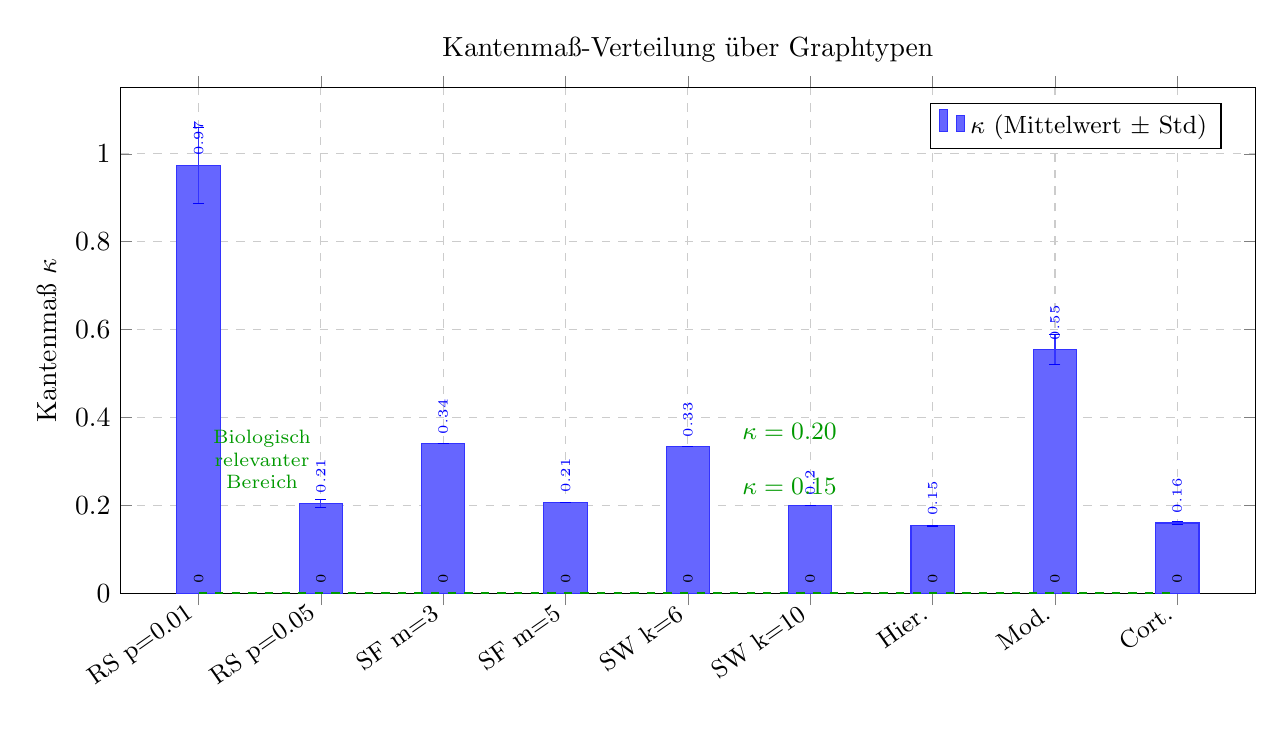
\begin{tikzpicture}
\begin{axis}[
    width=16cm,
    height=8cm,
    ybar,
    bar width=0.55cm,
    enlarge x limits=0.08,
    ylabel={Kantenma\ss{} $\kappa$},
    title={Kantenma\ss-Verteilung \"{u}ber Graphtypen},
    symbolic x coords={
        RS p=0.01,
        RS p=0.05,
        SF m=3,
        SF m=5,
        SW k=6,
        SW k=10,
        Hier.,
        Mod.,
        Cort.
    },
    xtick=data,
    x tick label style={rotate=35, anchor=east, font=\small},
    nodes near coords,
    nodes near coords align={vertical},
    every node near coord/.append style={font=\tiny, rotate=90, anchor=west},
    ymin=0,
    ymax=1.15,
    grid=major,
    grid style={dashed, gray!40},
    legend pos=north east,
    legend style={font=\small},
]

% Green shading for biological region [0.15, 0.20]
\addplot [draw=none, fill=green!20, forget plot]
    coordinates {(RS p=0.01,0) (RS p=0.05,0) (SF m=3,0) (SF m=5,0) (SW k=6,0) (SW k=10,0) (Hier.,0) (Mod.,0) (Cort.,0)};

% Bars with error
\addplot+[
    fill=blue!60,
    draw=blue!80,
    error bars/.cd,
    y dir=both,
    y explicit,
] coordinates {
    (RS p=0.01, 0.973) +- (0, 0.086)
    (RS p=0.05, 0.205) +- (0, 0.009)
    (SF m=3,   0.340) +- (0, 0.000)
    (SF m=5,   0.206) +- (0, 0.000)
    (SW k=6,   0.333) +- (0, 0.000)
    (SW k=10,  0.200) +- (0, 0.000)
    (Hier.,    0.154) +- (0, 0.001)
    (Mod.,     0.554) +- (0, 0.034)
    (Cort.,    0.160) +- (0, 0.004)
};
\addlegendentry{$\kappa$ (Mittelwert $\pm$ Std)}

% Horizontal lines for biological region
\draw[green!60!black, thick, dashed] 
    ({rel axis cs:0,0} -| {axis cs:RS p=0.01,0.15}) -- 
    ({rel axis cs:1,0} -| {axis cs:Cort.,0.15})
    node[right, font=\small, green!60!black] {};
\draw[green!60!black, thick, dashed] 
    ({rel axis cs:0,0} -| {axis cs:RS p=0.01,0.20}) -- 
    ({rel axis cs:1,0} -| {axis cs:Cort.,0.20})
    node[right, font=\small, green!60!black] {};

\end{axis}

% Label for green region
\node[green!60!black, font=\small] at (8.5, 2.05) {$\kappa = 0.20$};
\node[green!60!black, font=\small] at (8.5, 1.35) {$\kappa = 0.15$};
\node[green!60!black, font=\scriptsize, align=center] at (1.8, 1.7) 
    {Biologisch\\relevanter\\Bereich};

\end{tikzpicture}
\end{document}
